% Compiler ce document 

% package de base
\documentclass[10pt,a4paper]{article}
\usepackage[utf8]{inputenc}
\usepackage{listings}

% langues
\usepackage[usenames,dvipsnames]{xcolor}
\usepackage[francais]{babel}
\usepackage[T1]{fontenc}
\usepackage{amsmath}
\usepackage{amsfonts}
\usepackage{amssymb}
\usepackage{graphicx}
\usepackage{tabularx}
\usepackage{colortbl}
\usepackage[hyphens]{url}
\usepackage[hidelinks]{hyperref} % liens
\usepackage{fancyhdr} % En tetes / bas de page
\usepackage{helvet} % police helvetica
\usepackage{xcolor} % Style pour affichage du C
\usepackage{courier} % police pour les listings

\usepackage{listingsutf8}

% Page de Garde -- Necessite d'installer le package titling, si probleme
% commenter la ligne suivante ainsi que les infos necessaires a la page
% de garde
\usepackage{pageGarde/Garde_perso}

% commande pour faire des sections sans nombre 
% tout en la rajoutant dans la table des matières
\newcommand\sectionWithoutNumber[1]{\section*{#1} \addcontentsline{toc}{section}{\protect\numberline{}#1}}
\newcommand\subsectionWithoutNumber[1]{\subsection*{#1} \addcontentsline{toc}{subsection}{\protect\numberline{}#1}}
\newcommand\subsubsectionWithoutNumber[1]{\subsection*{#1} \addcontentsline{toc}{subsubsection}{\protect\numberline{}#1}}
% définition de nouvelles couleurs
\definecolor{lightblue}{rgb}{0.8,0.8,0.9}
\definecolor{grossblue}{rgb}{0,0,0.7}
%marge des pages
\setlength{\textwidth}{16cm}
\setlength{\textheight}{24cm}
\setlength{\oddsidemargin}{0cm}
\setlength{\voffset}{-1.5cm}
\setlength{\headheight}{15pt}

% set la police en arial
%% Sans-serif Arial-like fonts
\renewcommand{\rmdefault}{phv} 
\renewcommand{\sfdefault}{phv} 
\usepackage{tabularx}
\usepackage{graphicx}
\usepackage{eurosym}
\usepackage{xspace}
\newcommand{\projectname}[0]{LTANR\xspace} 

% configuration pour des listings
\lstset{ 
  showspaces=false,      
  showstringspaces=false, 
  showtabs=false,               
  tabsize=3,                     
  numbers=left
}

%enlève indentation en début de paragraphe
\setlength\parindent{0pt}

%style de l'en-tête de page
\pagestyle{fancy}

% style pour code en c
\lstdefinestyle{customc}{
  belowcaptionskip=1\baselineskip,
  breaklines=true,
  frame=L,
  xleftmargin=\parindent,
  language=C,
  showstringspaces=false,
  basicstyle=\scriptsize\ttfamily,
  keywordstyle=\bfseries\color{green!40!black},
  commentstyle=\itshape\color{purple!40!black},
  identifierstyle=\color{blue},
  stringstyle=\color{orange},
}

\lstdefinelanguage{VHDL}{
      morekeywords=[1]{
        library,use,all,entity,is,port,in,out,end,architecture,of,
        begin,and,or,Not,downto,ALL
      },
      morekeywords=[2]{
        STD_LOGIC_VECTOR,STD_LOGIC,IEEE,STD_LOGIC_1164,
        NUMERIC_STD,STD_LOGIC_ARITH,STD_LOGIC_UNSIGNED,std_logic_vector,
        std_logic
      },
      morecomment=[l]--
    }
    \usepackage[usenames,dvipsnames]{xcolor}
    \colorlet{keyword}{blue!100!black!80}
    \colorlet{STD}{Lavender}
    \colorlet{comment}{green!80!black!90}
    \lstdefinestyle{vhdl}{
      language     = VHDL,
      basicstyle   = \footnotesize \ttfamily,
      keywordstyle = [1]\color{keyword}\bfseries,
      keywordstyle = [2]\color{STD}\bfseries,
      commentstyle = \color{comment}
      breaklines=true,                % sets automatic line breaking
      tabsize=3                                % sets default tabsize to 2 spaces
    }

\lstset{escapechar=@,style=customc}
\lstset{inputencoding=utf8/latin1} %affiche les accents dans le listing

% Mise en forme de la page de titre
\author{João Miguel Domingues Pedrosa \\ Loïc Haas}
\title{Threading Building Blocks}
\dest{}

% Informations necessaires a la page de garde
% Commenter si probleme de compilation
\acro{HPC}
\matter{High Performance Coding}
\date{\today}

%en-tête
\lhead{Domingues \& Haas}
\chead{TBB}
\rhead{\theAcro}

%pied-de-page
\lfoot{HEIG-VD}
\cfoot{\today}
\rfoot{\thepage}

\begin{document}
\maketitle
\newpage
\tableofcontents
\newpage

%Ici commence réelement l'écriture du rapport

\section{Introduction}
L'objectif de ce projet est de comprendre, essayer et exploiter un outil d'optimisation. Dans notre cas, nous avons choisi TBB (Threading Building Blocks). Il s'agit d'une libraire d'Intel fait pour du C++. \\

Sa caractéristique est de simplifier au maximum l'implémentation de programme parallèle pour des systèmes multicœur. Le programmeur pourra ainsi faire un programme portable car c'est la librairie qui va se charger d'utilisé la bonne implémentation de thread (exemple: POSIX pour linux ou les threads Windows). Pour cela, elle met en place différentes fonction et objet lié à la programmation parallèle et à la gestion de concurrence.\\

Pour ce projet, nous avons du faire l'installation de la libraire, la procédure sera expliqué plus loin dans le rapport. Il y aura aussi un code exemple auquel on aura fait des mesures de performances afin de voir les optimisation apporté. Nous finirons par une analyse de notre constats tout au long de nos essaies.
\newpage

\section{Installation}
L'installation des libraires a été fait sur des machines possédant un OS Linux Ubuntu. Les installations suivantes ont été via ligne de commande.

\subsection{Installation via apt-get}

Pour installer sur nos machines, nous avons utilisé le gestionnaire de package \texttt{apt-get}. Le package installé est \texttt{libtbb2}. Cela nous donc la commande suivante:\\

\texttt{sudo apt-get install libtbb2}\\

Une fois installer, on peut commencé à programmer avec les librairies pthreads. Pour testé l'installation, on va compiler et exécuter un code exemple afin de voir s'il n'y a pas de problème.(commande pour la compilation \texttt{g++ <filename>.cpp -ltbb} )

\subsubsection{Code exemple}
\lstinputlisting{../test/test.cpp}

\newpage

\subsection{Installation via l'archive}

\begin{enumerate}

	\item Il faut premièrement télécharger. Pour cela, il faut se rendre sur le site d'Intel pour TBB et aller dans la section download\footnote{\url{https://www.threadingbuildingblocks.org/download}}. Ensuite, on copie l'adresse sur la release et l'OS que l'on veut (dans notre cas Linux). On entre ensuite la commande suivante:\\
	\texttt{\$ wget https://www.threadingbuildingblocks.org/sites/default/files/\linebreak software\_releases/linux/tbb<version>.tgz}
	
	\item Maintenant que l'on a télécharger l'archive, il faut l'extraire pour cela on fait la commande suivante:\\
	\texttt{\$ tar zxf tbb<version>.tgz}
	\item Un fois extrait, il faut se rendre dans le dossier \texttt{bin} et modifier le script \texttt{tbbvars.sh}. Il faut changer la ligne suivante:\\
	\texttt{TBBROOT = SUBSTITUTE\_INSTALL\_DIR\_HERE} \\
	par\\
	\texttt{TBBROOT = <path\_tbb\_directory>}\\
	Cela permettra lors de pouvoir utilisé la librairie facilement lors de la compilation.
	\item Après, on exécute le script avec la bonne option (ia32 pour une architecture 32 bits ou intel64 pour du 64 bits) et on peut commencé à fait des programme avec TBB.
	\item Pour tester si tout a été bien installer, on compile le code précédent et on l'exécute.
	Si il n'y a pas eu de problème durant la compilation et l'exécution c'est que tout est bon
\end{enumerate}

\begin{figure}[hpl]
	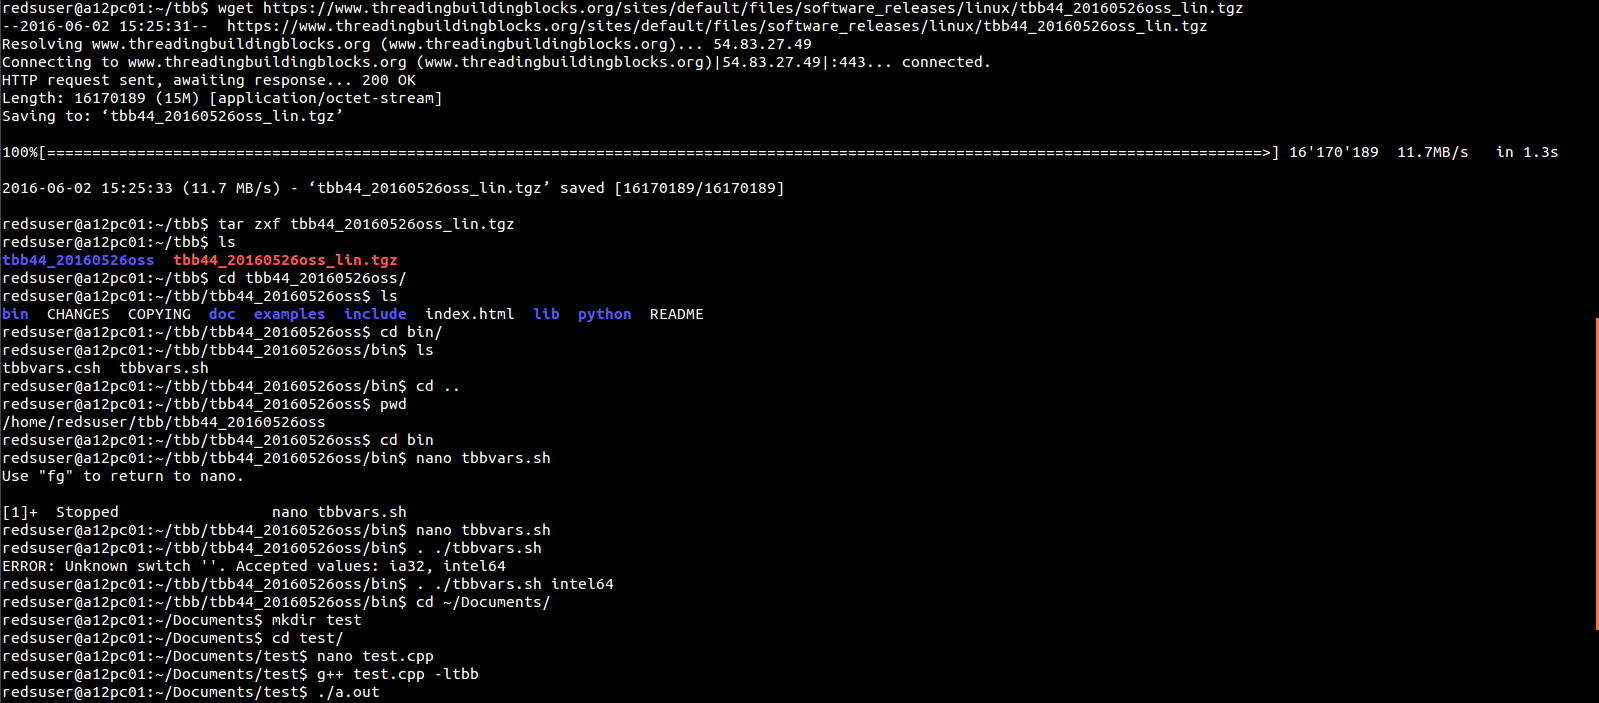
\includegraphics[width=\textwidth]{images/installcommands.png}
	\caption{Capture d'écran des commandes utilisées}
\end{figure}

\newpage

\section{Exemple}
Le programme utilisé pour l'exemple s'occupe de convertir une image couleur en une avec des nuances de gris. Nous avons choisi le code suivant car il se prête bien à la parallélisation et que nous avons déjà fait des optimisation avec d'autre outils. Cela nous permet ainsi de faire des meilleurs critiques au niveau des performances.

\subsection{Code}
% inserer le code ici

\subsection{Mesures}
 
\newpage

\section{Analyse}

\newpage

\section{Bibliographie}
\begin{itemize}
	\item Tutoriel d'Intel: \url{https://www.threadingbuildingblocks.org/intel-tbb-tutorial}
	\item Documentation d'Intel: \url{https://software.intel.com/en-us/tbb-documentation}
\end{itemize}

\end{document}
